\documentclass[border=10pt]{standalone}
\usepackage{tikz}
\usepackage{amsmath}
\usetikzlibrary{shapes.geometric, arrows, positioning}

\begin{document}

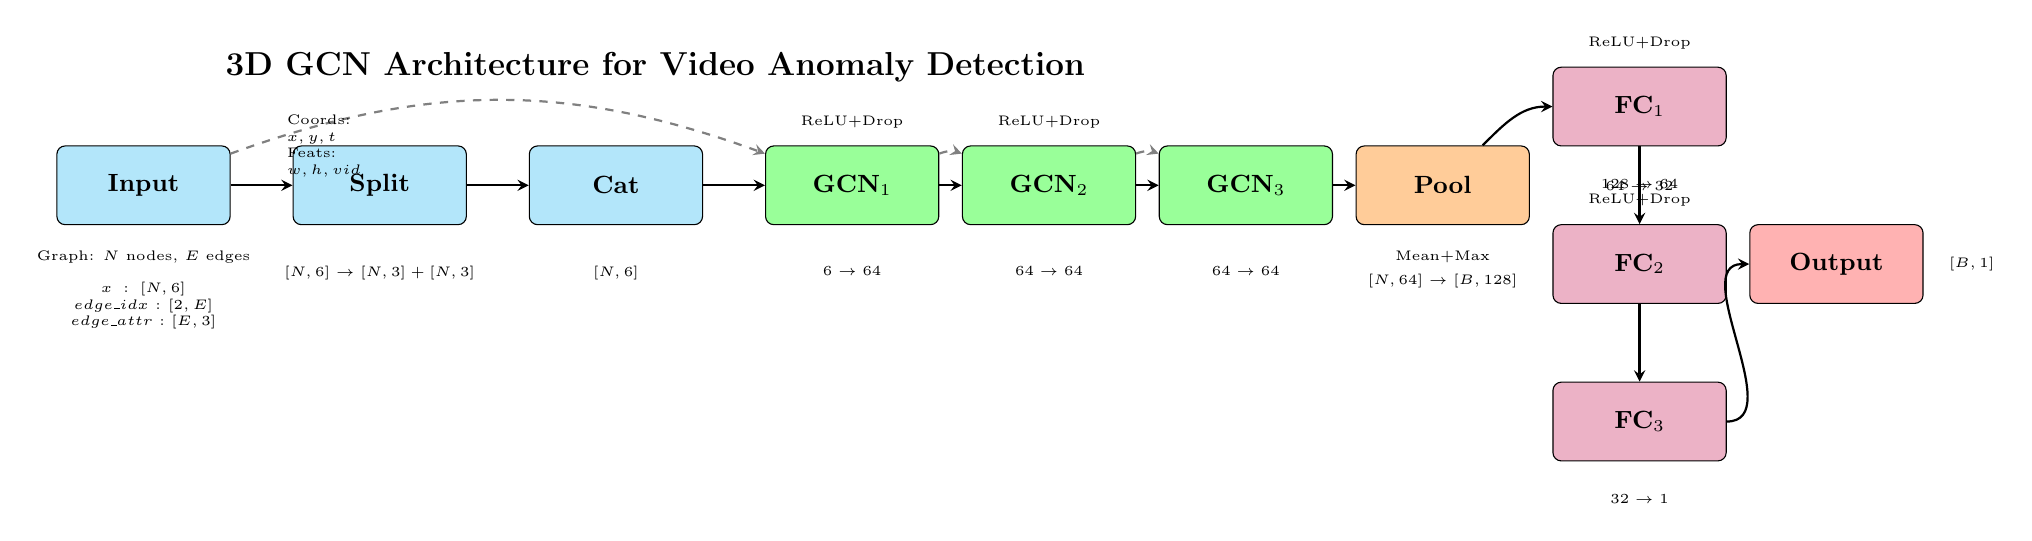
\begin{tikzpicture}[
    node distance = 1.2cm and 0.8cm,
    box/.style = {rectangle, rounded corners=3pt, minimum width=2.2cm, minimum height=1cm, 
                  text centered, draw=black, font=\small},
    input/.style = {box, fill=cyan!30},
    gcn/.style = {box, fill=green!40},
    pool/.style = {box, fill=orange!40},
    fc/.style = {box, fill=purple!30},
    output/.style = {box, fill=red!30},
    arrow/.style = {thick,->,>=stealth}
]

    % Title
    \node[font=\large\bfseries] (title) at (6.5,6) {3D GCN Architecture for Video Anomaly Detection};

    % Input
    \node[input] (input) at (0,4.5) {\textbf{Input}};
    \node[below=0.2cm of input, font=\tiny] {Graph: $N$ nodes, $E$ edges};
    \node[below=0.6cm of input, font=\tiny, text width=2cm, align=center] {
        $x: [N, 6]$\\
        $edge\_idx: [2, E]$\\
        $edge\_attr: [E, 3]$
    };

    % Feature extraction
    \node[input] (split) at (3,4.5) {\textbf{Split}};
    \node[below=0.4cm of split, font=\tiny] {$[N,6] \to [N,3]+[N,3]$};

    \node[input] (cat) at (6,4.5) {\textbf{Cat}};
    \node[below=0.4cm of cat, font=\tiny] {$[N, 6]$};

    % GCN Layers
    \node[gcn] (gcn1) at (9,4.5) {\textbf{GCN$_1$}};
    \node[below=0.4cm of gcn1, font=\tiny] {$6 \to 64$};

    \node[gcn] (gcn2) at (11.5,4.5) {\textbf{GCN$_2$}};
    \node[below=0.4cm of gcn2, font=\tiny] {$64 \to 64$};

    \node[gcn] (gcn3) at (14,4.5) {\textbf{GCN$_3$}};
    \node[below=0.4cm of gcn3, font=\tiny] {$64 \to 64$};

    % Pooling
    \node[pool] (pool) at (16.5,4.5) {\textbf{Pool}};
    \node[below=0.2cm of pool, font=\tiny] {Mean+Max};
    \node[below=0.5cm of pool, font=\tiny] {$[N,64] \to [B,128]$};

    % Classifier
    \node[fc] (fc1) at (19,5.5) {\textbf{FC$_1$}};
    \node[below=0.3cm of fc1, font=\tiny] {$128 \to 64$};

    \node[fc] (fc2) at (19,3.5) {\textbf{FC$_2$}};
    \node[above=0.3cm of fc2, font=\tiny] {$64 \to 32$};

    \node[fc] (fc3) at (19,1.5) {\textbf{FC$_3$}};
    \node[below=0.3cm of fc3, font=\tiny] {$32 \to 1$};

    % Output
    \node[output] (output) at (21.5,3.5) {\textbf{Output}};
    \node[right=0.2cm of output, font=\tiny] {$[B,1]$};

    % Main flow arrows
    \draw[arrow] (input) -- (split);
    \draw[arrow] (split) -- (cat);
    \draw[arrow] (cat) -- (gcn1);
    \draw[arrow] (gcn1) -- (gcn2);
    \draw[arrow] (gcn2) -- (gcn3);
    \draw[arrow] (gcn3) -- (pool);
    \draw[arrow] (pool) to[out=45, in=180] (fc1);
    \draw[arrow] (fc1) -- (fc2);
    \draw[arrow] (fc2) -- (fc3);
    \draw[arrow] (fc3) to[out=0, in=180] (output);

    % Edge index flow (dashed)
    \draw[arrow, dashed, gray] (input) to[out=20, in=160] (gcn1);
    \draw[arrow, dashed, gray] (gcn1) to[out=20, in=160] (gcn2);
    \draw[arrow, dashed, gray] (gcn2) to[out=20, in=160] (gcn3);

    % Features annotation
    \node[right=0.2cm of input, font=\tiny, text width=1.5cm] at (1.5,5) {
        Coords: $x,y,t$\\
        Feats: $w,h,vid$
    };

    % Activations
    \node[above=0.1cm of gcn1, font=\tiny] {ReLU+Drop};
    \node[above=0.1cm of gcn2, font=\tiny] {ReLU+Drop};
    \node[above=0.1cm of fc1, font=\tiny] {ReLU+Drop};
    \node[above=0.1cm of fc2, font=\tiny] {ReLU+Drop};

\end{tikzpicture}

\end{document}

